\section{Conceptos Preliminares}
\subsection{Acervo Genético, y Poblaciones Monomórficas y Dimórficas.}

La \textit{reserva genética} o \textit{acervo genético} de una población se define como los alelos\footnote{Un alelo es una de las versiones de una secuencia de ADN que se encuentra en una posición determinada de un cromosoma} de los genes encontrados en los individuos. Cada gen, a su vez, puede contar con su propio acervo genético, el cuál es constituido por lo alelos del mismo. Un ejemplo de esto es una población en la que cada individuo puede ser considerado como un ser único desde el punto de vista genético. Para cada alelo podríamos determinar la frecuencia de aparición, cantidad a la que llamamos frecuencia génica, y esta puede ser expresada como un porcentaje y representa la abundancia del alelo en relación a las otras versiones del su correspondiente gen. Supongamos una población con distintos tipos de alelos del gen $A$, digamos $A$y $A'$, el caso de ser sólo dos. Si esta población cuenta con 100 individuos, estos existen 200 alelos. Suponiendo que aparecen 120 alelos $A$ y 80 alelos $A'$, entonces las frecuencias génicas son 60\% y 40\% respectivamente.

Bajo este entendido, decimos que una población es genéticamente estable, o está en equilibrio genético, cuándo el acervo genético se mantiene constante en el tiempo. Si por el contrario, el acervo cambia de una generación a otra, la población está en \textit{trance evolutivo}. Así pues, las poblaciones genéticamente estables son una hipótesis. Estas fueros descritas por Hardy y Weinberg en 1908, quienes postularon que para que esto se cumpla, deben mantenerse las siguientes condiciones:

\begin{itemize}
	\item

	      La población deber ser muy grande, tal que un cambio fortuito no tenga impacto en su composición genética.



	\item

	      El apareamiento debe ser al azar, esto con motivo de que no haya \textit{favoritismo} hacia ciertas características, que son las que serán heredadas.



	\item

	      No debe haber mutaciones para que el acervo genético no cambie.



	\item

	      No debe haber selección natural, por lo que todos los genotipos\footnote{El genotipo es el conjunto de genes y la información genética que caracteriza a un individuo, y que se transmite de generación en generación} están en igualdad de condiciones con respecto a la reproducción y a la adaptación ambiental.



	\item

	      No debe haber migraciones, es decir, no debe haber flujo genético ni hacia dentro ni hacia afuera de la población.
\end{itemize}

No es difícil deducir qué condiciones deben darse para que la población entre en trance evolutivo.

\begin{itemize}
	\item

	      Poblaciones pequeñas.



	\item

	      Apareamiento selectivo.



	\item

	      Presencia de mutaciones.



	\item

	      Selección natural.



	\item

	      Migraciones, tanto internas como externas.


\end{itemize}

Puestos en este contexto podemos definir a las poblaciones monomórficas y dimórficas.

\textbf{Población Monomórfica:} decimos que una población es monomórfica cuando ésta presenta un sólo alelo para un gen específico. En este contexto decimos que todos los individuos son genéticamente idénticos respecto a dicho gen.

\textbf{Población Dimórfica:} decimos que una población es dimórfica cuando ésta presenta dos variaciones, o alelos en un gen específico.

Estas ideas pueden generalizarse a poblaciones polimórficas, siendo éstas aquellas que presentan un dos o más variaciones, o alelos, de un gen en partícular, pero a efectos de este trabajo, sólo nos resultarán de interés las monomórficas, y las dimórficas.

\subsection{\textit{Chemostat}}

El \textit{chemostat} o \textit{quimiostato} es un dispositivo de laboratorio que está diseñado para el estudio del crecimiento de microorganismos en un ambiente controlado, en un medio líquido. Este dispositivo funciona de la siguiente forma: a un recipiente de vidrio cerrado, de entre 1 mL y unos pocos litros, se le suministra un medio fresco a través de una bomba de afluente. Para mantener un volumen constante, una segunda bomba extrae el líquido a la misma velocidad. Los microorganismos que han sido añadidos al recipiente únicamente pueden alimentarse del la bomba de afluente, y la tasa de crecimiento de esta está definida como la relación entre la tasa de afluente y el volumen del recipiente. Entre los sustratos y factores de crecimiento añadidos al medio, uno es el llamado sustrato de control, que limita el crecimiento.

\begin{center}
	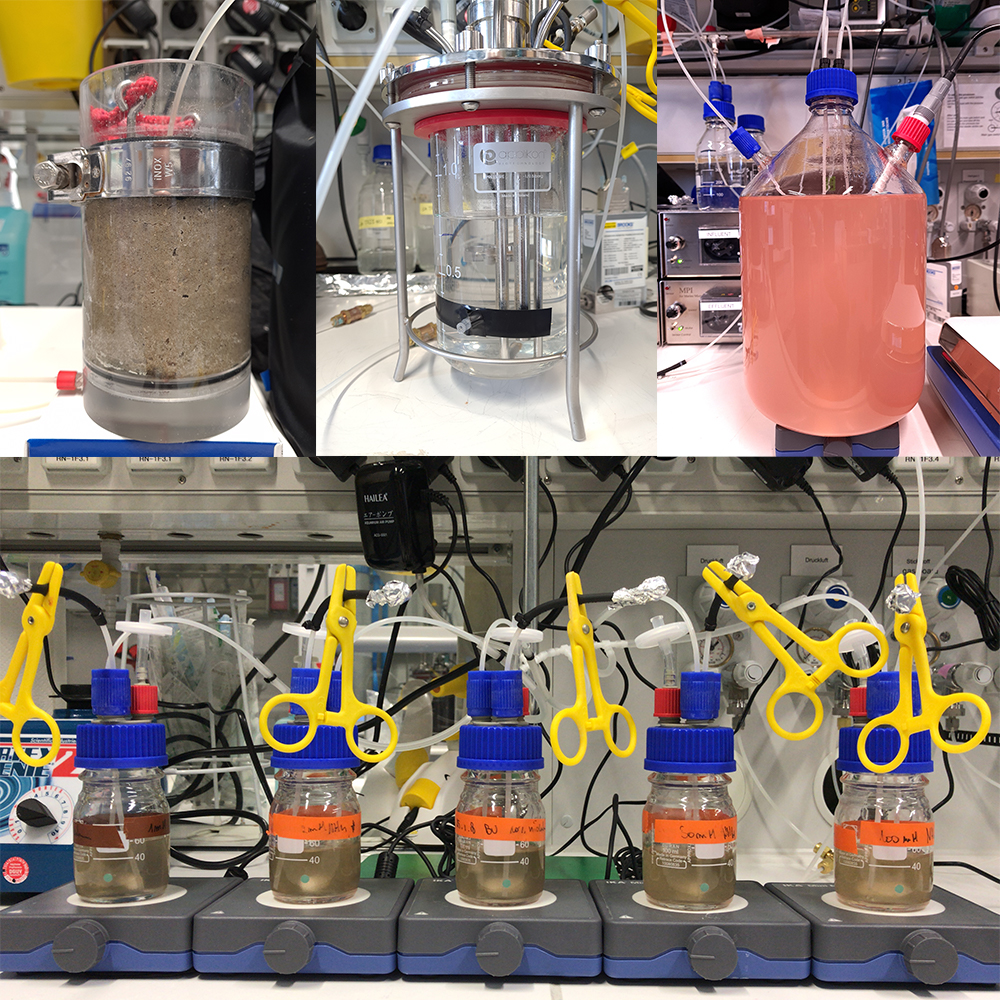
\includegraphics[scale=0.2]{Chemostat.jpg}
\end{center}

Un quimiostato es una buena opción para el cultivo de microorganismos, ya que establecemos condiciones que permanecen constantes, contra los cultivos hechos en lotes. Esto facilita enormemente la reproducción de los experimentos. Algunas de las utilidades del quimiostato son que puede ser utilizado en cultivos puros para el estudio de la cinética del crecimiento microbiano, o para enfoques ómicos más detallados. También se puede utilizar para experimentos de competición.

En estos experimentos se liberan en el recipiente dos o tres microorganismos diferentes, con nichos comparables en condiciones variables; con tasas de crecimiento altas o bajas; con concentraciones de oxígeno altas o bajas; distintos valores de pH o temperatura; con o sin factores de crecimiento, etc.

\subsubsection{GREENT}

La  actividad humana ha tenido serios impactos en los ciclos biológicos del carbono y nitrógeno, y como consecuencia, el calentamiento global y la contaminación del agua. En este contexto, las tecnologías relacionadas con el tratamiento de agua ha mejorado en las últimas décadas. En particular, el uso de anammox (bacterias anaeróbicas oxidantes de amonio) en gránulos con oxígeno tiene el potencial de convertir las tratadoras de agua en sistemas enérgicamente eficientes con mínima emisión de gases de efecto invernadero.

Existen microorganismos que acoplan la oxidación anaeróbica del metano con la desnitrificación. Una integración innovadora de estos en determinados sistemas de tratamiento de aguas podría ofrecer una solución elegante y eficiente para combatir las emisiones de gases de efecto invernadero de las mismas.

El propósito del \textit{GREENT}, o \textit{Mitigación de Gases de Efecto Invernadero Mediante Tecnología Avanzada de Eliminación de Nitrógeno} (por sus siglas en inglés) es determinar las emisiones de óxido nitroso en los bioreactores de nitritación parcial-anammox, y los parámetros que las gobiernan, e investigar las vías responsables con un detalle molecular. Aunado a ésto, también explorar la viabilidad de un bioreactor que elimine el amonio y metano de manera simultanea mediante anammox, y microorganismos anaeróbicos oxidantes de metano.

\subsection{Ecuación de Hamilton-Jacobi, Viscosidad y Constricciones.}